% Created 2014-11-10 Mon 23:54
\documentclass[9pt,b5paper]{article}
\usepackage{graphicx}
\usepackage{xcolor}
\usepackage{xeCJK}
\usepackage{longtable}
\usepackage{float}
\usepackage{textcomp}
\usepackage{geometry}
\geometry{left=0cm,right=0cm,top=0cm,bottom=0cm}
\usepackage{multirow}
\usepackage{multicol}
\usepackage{listings}
\usepackage{algorithm}
\usepackage{algorithmic}
\usepackage{latexsym}
\usepackage{natbib}
\usepackage{fancyhdr}
\usepackage[xetex,colorlinks=true,CJKbookmarks=true,linkcolor=blue,urlcolor=blue,menucolor=blue]{hyperref}


\lstset{language=c++,numbers=left,numberstyle=\tiny,basicstyle=\ttfamily\small,tabsize=4,frame=none,escapeinside=``,extendedchars=false,keywordstyle=\color{blue!70},commentstyle=\color{red!55!green!55!blue!55!},rulesepcolor=\color{red!20!green!20!blue!20!}}
\author{Jenny Huang}
\date{\today}
\title{Android App Programming Directed Study \textasciitilde{} DrawingFun}
\hypersetup{
  pdfkeywords={},
  pdfsubject={},
  pdfcreator={Emacs 24.3.1 (Org mode 8.2.7c)}}
\begin{document}

\maketitle
\tableofcontents


\section{first checkin 10/27/2014}
\label{sec-1}
\subsection{Goal}
\label{sec-1-1}
\begin{itemize}
\item According to the instructor's requirements that we are going to implement an simple window's Paint like Android app for later on integrating Unicon's 2D graphics to Android app.
\end{itemize}
\subsection{Course Introduction}
\label{sec-1-2}
\begin{itemize}
\item We have only two students, the other one is an udnergraduate exchange students with solid Java programming background and relatively slightly week problem-solving skills. For the first more than half semester, we used Sudoku as the starting point and tried several different topics to get our hands wet.
\end{itemize}
\subsection{Project Introduction}
\label{sec-1-3}
\begin{itemize}
\item It's after middle term already, the way we were currently trying on to make it work may just work perfectly for the other classmate, but for me, I feel like it takes forever for me to be able to make any significant progress. So about half a month ago, I was motivated and thought instead of surfacing around and having fun learning by trial and error, maybe I should start from an simple GUI app as a starting point and try my best to expend/extend the APP functionality from there. And also we would be able to work to our final project slightly earlier.
\item This GUI will be my very second GUI interface that I have ever created for my Computer Science major, (this first one was an Python Tkinter GUI one week short project for plotting graphics with data abstracted from backend database during an internship;). And I guess it may still be slightly difficult for me to start write Android App code of my own line by line, so I simply searched internet, and trying an tutorial to make a working starting point Android Paint GUI. I integrated the codes from the reference link all together, fixed minor compile errors, and it worked!
\item This "Copied" GUI will serve as the starting point, and my functionality updates start from here, and I will update my progress for this project later on by week according to the instructor's requirements and suggestions.
\end{itemize}
\subsection{References}
\label{sec-1-4}
\begin{itemize}
\item \url{http://code.tutsplus.com/tutorials/android-sdk-create-a-drawing-app-interface-creation--mobile-19021}
\end{itemize}
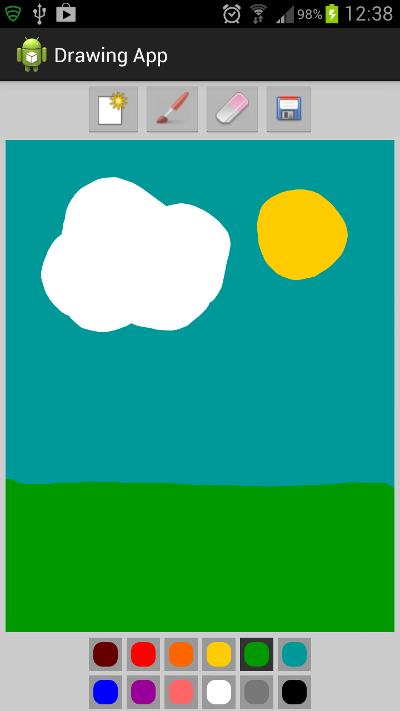
\includegraphics[width=.5\linewidth]{./android_drawing_final.png}

\section{Checkin for 11/3/2014}
\label{sec-2}
\subsection{Buttons I have worked on}
\label{sec-2-1}
\subsubsection{Color$_{\text{Picker}}$:}
\label{sec-2-1-1}
\subsubsection{Undo/Redo:}
\label{sec-2-1-2}

\subsection{Functionalities and References}
\label{sec-2-2}
\subsubsection{Color$_{\text{Picker}}$:}
\label{sec-2-2-1}
\begin{itemize}
\item Motivated by the Picasso Android app, seeing their multiple color choices, our starting point \textbf{12} fixed colors were too limited.
\end{itemize}
\subsubsection{Undo/Redo Buttons:}
\label{sec-2-2-2}
\begin{itemize}
\item Also motivated by the Picasso app, intended to work on \textbf{Undo} button, and ended up found \textbf{Redo} button could be very convenient as well.
\item needs to update these Undo/Redo methods later on, this is just the starting point most basic implementation for this button set.
\end{itemize}
\subsubsection{Snapshot}
\label{sec-2-2-3}
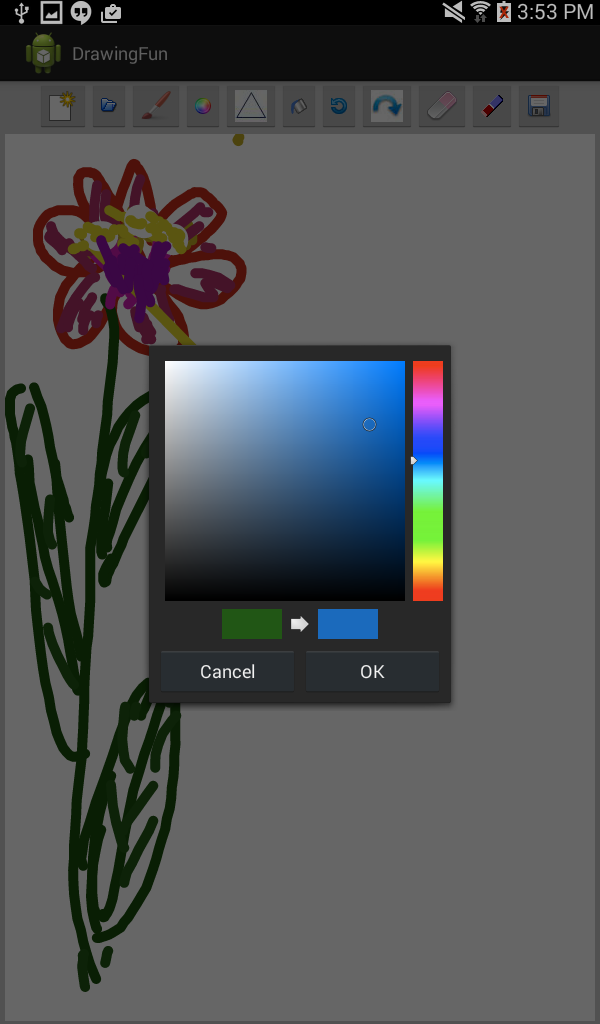
\includegraphics[width=.5\linewidth]{./20141103.png}

\subsection{Todo}
\label{sec-2-3}
\begin{itemize}
\item Drawing shapes with Finger for primitives: refer to the reference below: \url{http://gmariotti.blogspot.com/2014/01/drawing-shapes-with-fingers.html}. This button will be first priority to finish.
\item Load image file button
\item Erase Rectangle
\item Undo/Redo
\end{itemize}

\section{Checkin for 11/10/2014}
\label{sec-3}
\subsection{Buttons I have worked on}
\label{sec-3-1}
\begin{itemize}
\item shapeBtn for primitives
\end{itemize}

\subsection{Functionalities and References}
\label{sec-3-2}
\subsubsection{shapeBtn for primitives: Drawing shapes with Finger for primitives}
\label{sec-3-2-1}
\begin{itemize}
\item refer to the reference below for some basic shapes: line, smooth line, circle, triangle, Rectangle, square
\item \url{http://gmariotti.blogspot.com/2014/01/drawing-shapes-with-fingers.html}
\item \textbf{ListView} in \textbf{Alert Dialog} is searched from online without direct reference.
\item Since the erase was using draw smooth line. This button works also means that I could erase a "\textbf{Rectangle}" shape, or "\textbf{Circle}" shape.
\item I have other course priority for the passed week, so I just have enough time to finish this course's priority, but I will try to work harder in order to finish all the functionalities for this course.
\item It's not a good looking ListView, but yet it's a fully functional button.
\item This button right now is fully functional, but to finish this project first, I have not spent any quality time to expand any primitives yet, rather than the existing six ones from the reference listed below.
\end{itemize}
\subsubsection{Snapshot}
\label{sec-3-2-2}
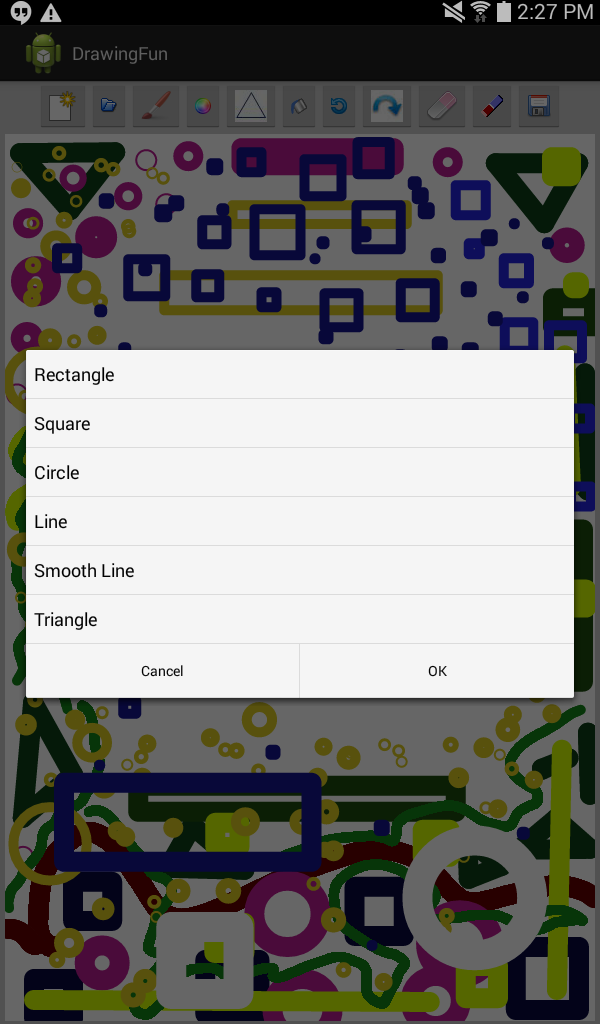
\includegraphics[width=.5\linewidth]{./20141110-14-27-05.png}
\subsection{Todo}
\label{sec-3-3}
Rank any one of the first three to be top priority, and go from there.
\begin{itemize}
\item Erase Rectangle
\item Undo/Redo
\item Fill paint
\item Load image file button
\end{itemize}
% Emacs 24.3.1 (Org mode 8.2.7c)
\end{document}